\section{Systematic Literature Review}

A systematic literature review is a type of review that aims to identify,
evaluate, and summarize the results of all studies that address a specific
research question or topic
\cite{kitchenham2007guidelines,kitchenham2009systematic,gough2017introduction}.
It involves following a specific methodology to identify, analyse, and
interpret all relevant evidence related to the research question being
addressed. The purpose of a systematic literature review is to provide a
comprehensive and up-to-date overview of the current state of knowledge on a
specific research question or topic. It is a critical appraisal of the existing
research and it can help identify gaps in the literature and inform future
research directions \cite{kitchenham2007guidelines}.

As per Kitchenham and Charters guidelines \cite{kitchenham2007guidelines}, a
systematic literature review (SLR) involves three phases: planning, conducting,
and reporting. The planning phase involves establishing the review protocol
based on the research questions and the need for the review. The conducting
phase involves selecting primary studies and applying the criteria established
in the review protocol to analyse them. Finally, the reporting phase involves
the creation of the report. These guidelines were loosely followed in the
development of this review.

\subsection{Research Methodology} \label{sub:research-methodology}

To address the research questions posed in \Cref{sec:introduction}, the
appropriate research methods were utilised as means to properly investigate the
current state of the art. To give guidance,
\Cref{fig:review-iterations} shows a diagram of the review iterations that will
be explained in the following sections.

\begin{figure*}[!htb]
  \caption{Review iterations}
  \label{fig:review-iterations}
  \centering
  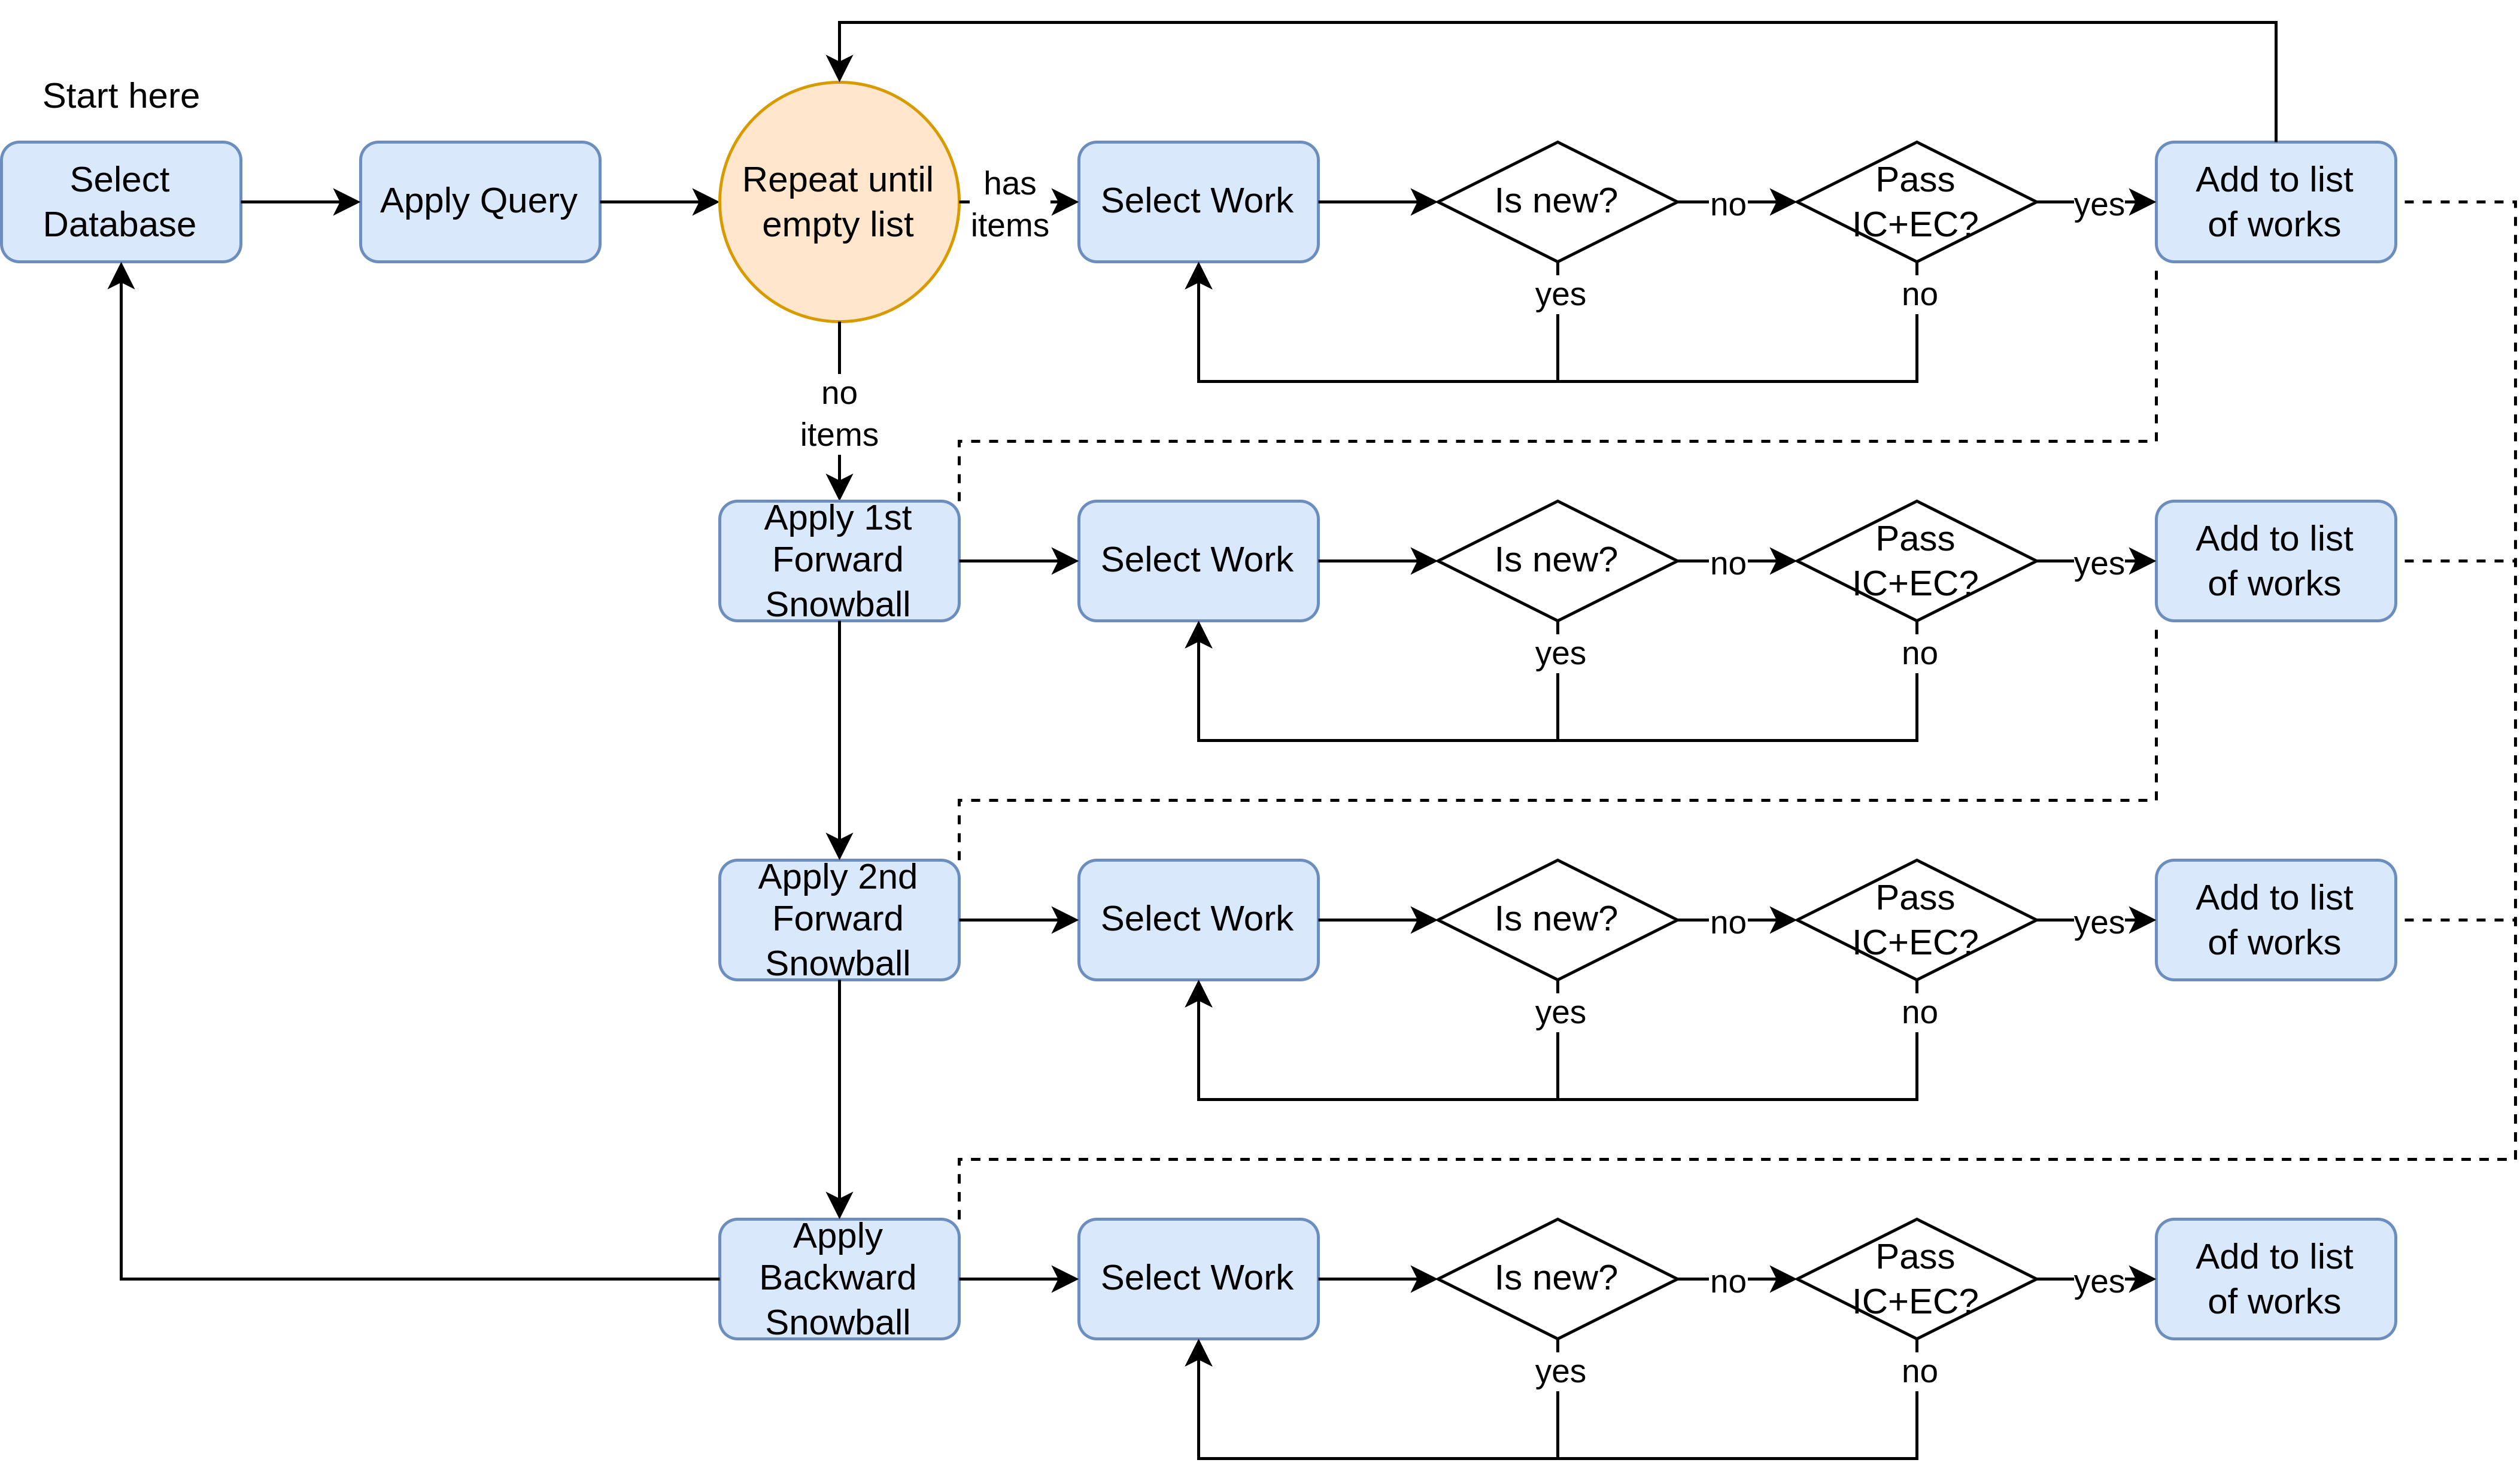
\includegraphics[width=\textwidth]{thesis-review-iterations.drawio}
\end{figure*}

\subsubsection{Data sources}

To access relevant research and information in this field, it is advisable to
search several databases that specialise in scientific literature.
\Cref{tab:databases} presents a list of several such databases, including the
ACM Digital Library, Science Direct, IEEE Xplore, Wiley, Springer Link,
Engineering Village, and Google Scholar. These databases contain a wealth of
knowledge and resources, including journal articles, conference proceedings,
technical reports, and more, which can be useful for staying up to date on the
latest developments in this field.

\begin{table}[!htb] \caption{Databases} \label{tab:databases}
  \begin{center}
    \begin{tabular}[c]{l|l|l} \textbf{ID} & \textbf{Search Engine} &
      \textbf{Website} \\
      \hline DB.1 & ACM Digital Library & \url{https://dl.acm.org/} \\
      \hline DB.2 & IEEE Xplore & \url{https://ieeexplore.ieee.org/} \\
      \hline DB.3 & Springer Link & \url{https://link.springer.com/} \\
      \hline DB.4 & Wiley & \url{https://onlinelibrary.wiley.com/} \\
      \hline DB.5 & Science Direct & \url{https://www.sciencedirect.com/} \\
      \hline DB.6 & Engineering Village &
      \url{https://www.engineeringvillage.com/} \\
      \hline DB.7 & Google Scholar & \url{https://scholar.google.com/} \\
    \end{tabular}
  \end{center}
\end{table}

\subsubsection{Search strategy}

To ensure a thorough and comprehensive search for relevant publications in this
field, we will utilise a breadth-first search approach. This method involves
starting with a specific query string and selecting relevant publications from
a given database. We will then use a technique called snowballing to expand the
search and locate additional relevant publications. Snowballing involves
searching for citations and publications that are related to the initially
selected publications.

There are two types of snowballing that we will employ in this search: forward
snowballing and backward snowballing. Forward snowballing involves searching
for citations and publications using Google Scholar for the initially selected
publications. This process can be repeated multiple times, with each iteration
referred to as a level of snowballing. For this search, we will
perform two levels of forward snowballing, in which we extract the references
of the initially selected publications (level one) and then select the
references of those references (level two).

Backward snowballing involves searching for publications that have been cited
by the initially selected publications. This technique can also be repeated
multiple times, but for this search, we will only perform one
level of backward snowballing. This will include all previous publications
found during the forward snowballing step.

By utilising both forward and backward snowballing techniques, we aim to cast a
wide net and identify as many relevant publications as possible.

After completing the search for relevant publications in a given database using
the specified query string, we will move on to the next database. This approach
is advantageous because it allows us to efficiently locate relevant
publications while minimizing the number of duplicates that are analysed. By
searching multiple databases and using snowballing techniques, we can identify
a large number of relevant publications and eliminate the need to analyse many
of them in subsequent iterations.

\subsubsection{Query definition}

To identify relevant publications for this research, we will utilise a range of
keywords related to the topic of microservices. These keywords will include
various phrases and terms used to describe microservices. As for the practices
that may help identification of microservices, keywords that help this
architectural refactoring should be included, such as ``migration",
``refactor", ``identification". It could also be useful to use ``monolith" (and
all its possible synonyms) to be the comparison against ``microservices",
although this can result in some extra publications not related to
microservices but instead related to ``service-oriented architecture". An
expected outcome or conclusion of the publication could be included,
``approach" or even ``tool". The main keywords that will be used are present in
\Cref{tab:keywords}.

\begin{table}[!htb] \caption{Keywords} \label{tab:keywords}
  \begin{center}
    \begin{tabular}[c]{p{7em}|p{13em}} {\textbf{Focus}} & microservices \\
      \hline \textbf{Refactoring} & {migration, decomposition, identify, refactor, evolve, discover, transition } \\
      \hline \textbf{Target} & monolith \\
      \hline \textbf{Outcome} & approach, tool \\
    \end{tabular}
  \end{center}
\end{table}

\subsubsection*{First iteration} \label{subsub:first-iteration}

The first iteration of the review has the main purpose of determining how many
tools exist that are able to solve this research question or, at the very
least, help partially with it. In order to do this, one could not be limited to
tools that are documented in academic databases therefore, in addition to the
databases mentioned in \Cref{tab:databases},
\href{https://github.com}{GitHub}, \href{https://gitlab.com}{GitLab} and even
\href{https://duckduckgo.org}{DuckDuckGo} were searched for, even though they
do not represent a scientific search engine.

By using some keywords mentioned in \Cref{tab:keywords} the following
initial trial query was created:

\begin{center}
  \emph{(``microservice" OR ``micro-service") AND (``migration" OR
  ``identification") AND (``monolithic" OR ``monolith") AND (``tool")}
\end{center}

\subsubsection*{Second iteration} \label{subsub:second-iteration}

In the second iteration of the review process, the focus is on locating
publications that describe alternative approaches for migrating from monolithic
to microservices architectures that may not have been implemented in practice.
This will allow an increased understanding of the current state of the art in
this area, identify any gaps or areas where further research is needed, and
determine what can be improved upon. This information will be useful in guiding
the development of our tool and abstraction.

As this was the beginning of a new iteration of the review process, the results
of the previous ``test run" were not considered when extracting literature.
Only after this iteration was completed did we incorporate the previously
analysed literature and exclude it from further analysis to avoid duplication
of effort. This allowed us to focus on identifying new and potentially relevant
publications for our purposes.

Relying on the keywords identified in \Cref{tab:keywords}, the following
query was created:

\begin{center}
  \emph{(microservice* OR micro?service*) AND (migrat* OR identif*) AND
  (monolith*) AND (migrat* NEAR/2 (process* OR approach*))}
\end{center}

In the event that the publications located through the snowballing approach are
no longer adding significant value to the overall understanding of the topic, a
new search query should be applied to the remaining databases. In some
instances, the query produced more than two thousand results, which would have
been impractical to analyse within the given timeframe. Therefore, we modified
the query to focus only on the titles and abstracts of the publications. The
revised query that should be used is:

\begin{center}
  \emph{(microservice* OR "micro-service") AND (migrat* OR decompos* OR
  identif* OR refactor* OR evolv* OR extract* OR discover* OR transition*)}
\end{center}

\subsubsection{Selection Criteria} \label{sub:selection-criteria}

In order to filter the publications, the title and the abstract will be
analysed and should mention at least one of:

\begin{enumerate}[{IC}1.]
  \item A tool that automates the process of migration of monoliths to
    microservices.
  \item Identification of microservices from monolith systems.
  \item Analysis of tools or approaches for migrating from monoliths to
    microservices.
\end{enumerate}

In cases of ambiguous abstracts, further inspection of the publication may be
done. When this happens, and if relevant publications apply, conclusions should
also be taken into account.

As for more pratical approach for exclusion of publications, the criteria will
be:

\begin{enumerate}[{EC}1.]
  \item Publications that are not written in English or Portuguese.
  \item For Portuguese publications, English must be the language used in the
    abstract.
  \item Publication is not accessible.
\end{enumerate}

\subsection{Research Results}

The query mentioned in the first iteration \Cref{subsub:first-iteration} was
then applied to DB.1, DB.2 and DB.3 and after applying the selection criteria
mentioned in \Cref{sub:selection-criteria}, results were gathered and
are presented in \Cref{tab:tool-search}.

\begin{table}[!htb] \caption{Tool Search} \label{tab:tool-search}
  \begin{center}
    \begin{tabular}[c]{p{5.5em}|p{5em}|p{5em}} \textbf{Database} &
      \textbf{Total\newline number\newline of results} &
      \textbf{Extracted\newline Results} \\
      \hline DB.1 & {118} & {3} \\
      \hline DB.2 & {4} & {0} \\
      \hline DB.3 & {658} & {3} \\
    \end{tabular}
  \end{center}
\end{table}

As for \href{https://github.com}{GitHub}, \href{https://gitlab.com}{GitLab} and
\href{https://duckduckgo.org}{DuckDuckGo}, the query would be essentially typed
into their respective search engine and the results gathered as well as the
query are presented in \Cref{tab:search-engine-tool-search}.

\begin{table}[!htb] \caption{Search Engine Tool Search}
  \label{tab:search-engine-tool-search}
  \begin{center}
    \begin{tabular}[c]{p{5.5em}|p{10em}|p{5em}|p{4em}}
      \textbf{Search\newline Engine} &
      \textbf{Query} &
      \textbf{Total\newline number\newline of results} &
      \textbf{Extracted\newline Results} \\
      \hline
        GitHub &
        \url{https://github.com/search?q=monolith+to+microservice} &
        {745} &
        {4} \\
      \hline
        GitLab &
        \url{https://gitlab.com/search?search=monolith\%20to\%20microservice} &
        {0} &
        {0} \\
      \hline
        DuckDuckGo &
        \url{https://duckduckgo.com/?q=monolith+to+microservices+tool} &
        {Uncountable} &
        {2} \\
    \end{tabular}
  \end{center}
\end{table}

Through this search process, we can also trace the references used in these
publications to determine if the tools described were based on previous work,
but only implemented a specific approach. This will help us to understand the
context and origins of these tools and how they fit into the broader landscape
of research in this area.

As for the second iteration mentioned in \Cref{subsub:second-iteration}, we
then proceeded to apply the query and search the first database. As shown in
\Cref{tab:db1-search}, from four hundred and fifty results, only twelve passed
the selection criteria defined in \Cref{sub:selection-criteria}.

\begin{table}[!htb] \caption{DB.1 Results} \label{tab:db1-search}
  \begin{center}
    \begin{tabular}[c]{p{5em}|p{5em}} \textbf{Total\newline number\newline of
      results} & \textbf{Extracted\newline New Results} \\
      \hline{450} & {12} \\
    \end{tabular}
  \end{center}
\end{table}

After reviewing the references of the identified papers and applying forward
and backward snowballing techniques, we were able to locate additional related
publications and expand the scope of our search as demonstrated in
\Cref{tab:db1-snowballing}. This helped us to increase the number of relevant
publications that we were able to consider in the next steps of the process.

\begin{table}[!htb] \caption{DB.1 Snowballing Results} \label{tab:db1-snowballing}
  \begin{center}
    \begin{tabular}[c]{p{8em}|p{8em}|p{8em}}
      \textbf{1st Forward} &
      \textbf{2nd Forward} &
      \textbf{Backward} \\
      \hline{23} &
      {2} &
      {45} \\
    \end{tabular}
  \end{center}
\end{table}

\begin{table}[!htb] \caption{Remaining DB Results} \label{tab:other-db-search}
  \begin{center}
    \begin{tabular}[c]{p{5em}|p{5em}|p{5em}}
      \textbf{Database} &
      \textbf{Total\newline number\newline of results} &
      \textbf{Extracted\newline New Results} \\
      \hline {DB.5 - 1st} & {21} & {1} \\
      \hline {DB.5 - 2nd} & {0} & {0} \\
      \hline {DB.4} & {9} & {3} \\
      \hline {DB.6} & {114} & {12} \\
      \hline {DB.3} & {20} & {0} \\
      \hline {DB.2} & {0} & {0} \\
    \end{tabular}
  \end{center}
\end{table}

In the case of Science Direct, as presented in \Cref{tab:other-db-search},
two queries were done. The main reason for this is that Science Direct is
limited to 7 \textit{OR} conditions, therefore it was necessary to split it
into two queries where it does not affect the general condition. In the
specific case, the \textit{``evolv"} keyword was moved into a separate query.
Also, Science Direct automatically accepts truncations without using the
\textit{``*"} char. The two queries are:

\begin{enumerate}
  \item \emph{(microservice OR "micro-service") AND ( migrat OR decompos OR
    identif OR refactor OR extract OR discover OR transition)}
  \item \emph{(microservice OR "micro-service") AND (evolv)}
\end{enumerate}

After iterating over the results and reviewing the references of the newly
found publications, we did not identify any additional publications that were
worth including in the final list. This marked the end of our general search
for relevant publications. We were able to find one hundred and six relevant
publications.

\subsection{Publications Grouping}

Given the large number of publications that were identified as potential
candidates for further analysis, it was necessary to further reduce the list to
a more manageable size. To accomplish this, we employed a categorization
approach in order to better organize and prioritize the publications for later
selection. This allowed us to select and analyse the most relevant publications
for our purposes. Through this process, we arrived at three main categories
that were derived from RQ1 into which we could place each publication. This
will be especially relevant when creating the new tool, by enhancing the
possibility of integrating various tools that employ different approaches, in
order to provide the developer with multiple perspectives, which may facilitate
the ability to make comparisons and informed decisions.

\begin{itemize}
  \item The \textbf{approach} used for identifying microservices from
    monoliths, \Cref{tab:approach-grouping}.
  \begin{itemize}
    \item \textit{Data flow}.
    \item \textit{Dependency analysis}.
    \item \textit{Execution log}.
    \item \textit{etc}.
  \end{itemize}
  \item The current \textbf{status} of the publication,
    \Cref{tab:status-grouping}.
  \begin{itemize}
    \item It only explains the \textit{method} at a high level.
    \item Has implementation details with the \textit{algorithm} on how to
      identify.
    \item Already has a working \textit{tool}.
  \end{itemize}
  \item The \textbf{language} in which that it targets,
    \Cref{tab:language-grouping}.
  \begin{itemize}
    \item \textit{Java}.
    \item \textit{Cpp}.
    \item \textit{C}.
    \item \textit{Language Agnostic}.
    \item \textit{etc}.
  \end{itemize}
\end{itemize}

The publications that were selected are grouped in
\Cref{tab:approach-grouping,tab:status-grouping,,tab:language-grouping}. It is
important to note that the papers analysed in this study were classified into
multiple categories, as opposed to a singular classification. To facilitate a
more comprehensive understanding, the classified papers can be viewed on the
online spreadsheet \footnote{\url{https://bit.ly/publication-grouping}}.

\begin{table}[!htb] \caption{Approach grouping} \label{tab:approach-grouping}
  \begin{center}
    \begin{tabular}[c]{p{12em}|p{4em}}
      \textbf{Approach} &
      \textbf{Amount} \\
      \hline Data flow & {8} \\
      \hline Control flow & {7} \\
      \hline Dynamic analysis & {11} \\
      \hline Semantic analysis & {4} \\
      \hline Problem frames & {1} \\
      \hline Model based & {10} \\
      \hline Static analysis & {13} \\
      \hline Dependency analysis & {15} \\
      \hline Multi objective & {1} \\
      \hline Feature analysis & {7} \\
      \hline Data analysis & {6} \\
      \hline REST & {4} \\
      \hline Graph based & {2} \\
      \hline Domain analysis & {10} \\
      \hline Neural analysis & {2} \\
      \hline Layer & {1} \\
      \hline Business analysis & {3} \\
      \hline Strangler pattern & {1} \\
      \hline Code change history & {1} \\
      \hline Contributor based & {1} \\
      \hline Logs analysis & {1} \\
      \hline Transactional contexts & {1} \\
      \hline Execution flow & {1} \\
      \hline Unknown & {2} \\
    \end{tabular}
  \end{center}
\end{table}

\begin{table}[!htb] \caption{Status grouping} \label{tab:status-grouping}
  \begin{center}
    \begin{tabular}[c]{p{12em}|p{4em}}
      \textbf{Status} &
      \textbf{Amount} \\
      \hline Method & {48} \\
      \hline Algorithm & {7} \\
      \hline Tool & {25} \\
      \hline Unknown & {1} \\
    \end{tabular}
  \end{center}
\end{table}

\begin{table}[!htb] \caption{Language grouping} \label{tab:language-grouping}
  \begin{center}
    \begin{tabular}[c]{p{12em}|p{4em}}
      \textbf{Language} &
      \textbf{Amount} \\
      \hline Agnostic & {59} \\
      \hline Java & {16} \\
      \hline Ruby & {1} \\
      \hline Python & {3} \\
      \hline Unknown & {4} \\
    \end{tabular}
  \end{center}
\end{table}

\subsection{Selected Work}

Having evaluated most of the literature in regard to tools that help with the
migration of monoliths to microservices, we need to select those that are most
relevant for the purpose of this thesis. Given our focus on tools and their
implementation, we will prioritise works that have already developed a tool and
made it available for a free inspection and use. Therefore, if a publication
does not provide a link to the tool or instructions for self-hosting or
deploying it, it is not worth further consideration. This will help us to focus
our efforts on publications that provide practical and useful information about
tools and their implementation.

\subsection{Publication Analysis} \label{sub:publication-analysis}

In the following sections, we will provide an analysis of the data collected
during the knowledge extraction process from the selected publications. This
analysis will allow us to address the primary research question (RQ1) and its
sub-questions.

\subsubsection{Monolith as an input for the tool}

The first aspect to be analysed is the input requirements for the tool. Despite
the growing interest in microservice migration using automated tools, the field
is still in its infancy, and the existing solutions tend to address specific
issues rather than being versatile. As a result, the inputs for these tools are
often rigid and not easily adjustable. For example, raw source code and OpenAPI
specification were possible ways tools use for identifying microservices from
monoliths and will be further discussed.

\subsubsection*{Source Code}

One potential method for providing input to a tool is by utilising source code
directly. Our research revealed that eighteen of the contributions analysed use
source code as input for their tools with multiple using Spring Boot or other
equivalent frameworks to help in understanding the overall code structure. One
reason for the use of frameworks is that they provide building blocks for
developers, meaning the core functionality of the framework is already in place
and developers simply fill in the gaps allowing for the framework to apply
inversion of control \cite{gamma1995design}. Since the behaviour of the
framework is kept intact, the tool can then safely analyse the overall code and
even apply the refactoring.

For instance, Freitas et al. \citeSLR{freitas2021refactoring} tool, MicroRefact
\footnote{\url{https://github.com/FranciscoFreitas45/MicroRefact}}, utilises
Java source code to extract structural information by relying on the Abstract
Syntax Tree. This information is used to generate a list of candidate
microservices. They then leverage Spring Boot decorators, particularly those
utilising the Java Persistence API (JPA), to infer the entities of the database
and their relationships. This process then results in the output of working
Java code for each identified microservice.

\subsubsection*{OpenAPI}

In a microservices architecture, one of the common solutions for communication
between different microservices is through HTTP calls. Therefore, it is
reasonable to assume that identifying microservices within a monolithic
application could be done by examining their REST endpoints since they will be
exposed through HTTP protocols. This inspection of REST endpoints can also
serve as a guide for decomposing the monolithic application into smaller,
independent services. In fact, when the programming language was not a
determining factor, OpenAPI was commonly used as the standard for
distinguishing microservices from monolithic systems.

The tool proposed by Al-Debagy and Martinek \citeSLR{al2019new} utilises the
OpenAPI specification file to identify microservices within a monolithic
application. The tool begins by extracting the operation names from the OpenAPI
file, which are then input into the Affinity Propagation Algorithm
\cite{frey2007clustering}. This algorithm calculates the number of
microservices by analyzing the messages exchanged between data points.
Afterwards, clustering is performed by utilising the Silhouette coefficient
\cite{rousseeuw1987silhouettes} which results in the identification and
grouping of similar microservices, helping in the decomposition of the
monolithic system.

MsDecomposer \footnote{\url{https://github.com/HduDBSI/MsDecomposer}}
\citeSLR{sun2022expert} uses a similar approach to identify microservices
within a monolithic application. The first step is to calculate the similarity
of candidate topics and response messages among the APIs. Then, it constructs a
graph that represents the similarity between different APIs, where the APIs are
represented as nodes and the similarity score is the weight. Finally, it
applies a graph-based clustering algorithm on the constructed graph, which
helps to identify the candidate microservices.

This highlights that OpenAPI is a language-agnostic method for identifying the
architecture of software systems.

\subsubsection*{Other}

Besides the input types that have been previously mentioned, there are other
types that may not be able to create a new category but are still relevant to
the microservices identification process. For example, using a specific system
model as input \citeSLR{staffa2021pangaea} or utilising the history of changes
to understand in addition to common artefacts like classes and methods
\citeSLR{santos2021microservice}.

\subsubsection{Microservices as an output for the tool}

For microservices identification, it is important to understand how existing
tools output their identified microservices in order to cater to the needs of
users. The ideal outcome would be a fully functional code ready to be deployed,
as it makes the migration process smoother, ensuring that the resulting
microservices have all the necessary components and reducing the effort needed
for manual migration. From the work that was analysed, tools that output a list
of candidates and tools that output source code are more relevant to take into
consideration and will be further discussed.

\subsubsection*{Candidates List}

A prevalent approach for identifying microservices in a monolithic system is by
producing a candidate list. This approach is used in most of the publications
and tools found, and it is a way of providing an organized and structured
output of the microservices that can be derived from the monolithic
application, in order to facilitate the migration process. The candidate list
is commonly used as a guide or checklist for architects, engineers, and
developers to assist in the actual partitioning of the application. It
typically includes but is not limited to, data entities, interfaces, methods,
and other relevant system components that are used as references to guide the
migration process.

The tool proposed by Al-Debagy and Martinek \citeSLR{al2019new} uses OpenAPI as
input to identify microservices within a monolithic application. One of the
limitations of their output is that it only provides a list of candidates,
which may not include information about the relationships and interactions
between each microservice. This can be an inconvenience when assigning
different development teams or groups with the task of applying the migration,
as they may not have enough information to understand how the microservices
interact and depend on each other, making it harder to assign and split the
workload accordingly.

There are other tools available that output a more informative result for
microservices identification. Even though they still output candidate lists,
where no migration is done yet, these tools provide more detailed information
about the relationships and connections between microservices, some of them
even including visual feedback such as clusters and call context tree diagrams
\citeSLR{krishna2021transforming, kalia2021mono2micro, kalia2020mono2micro,
nakazawa2018visualization}. This additional information can be very beneficial
for architects and developers, as it makes it easier for them to understand the
connections and dependencies between microservices, and make informed decisions
about how to proceed with the migration process.

\subsubsection*{Source Code}

Generating the final output of the migration process as source code that is
ready to be deployed would be the ideal outcome for most cases, as it would
lessen the efforts needed to migrate, but it is not yet commonly used in
current literature. Out of the tools that were analysed, only two of them
employ this method. One of them is the work of Freitas et al.
\citeSLR{freitas2021refactoring}, and another is Mono2Micro
\citeSLR{krishna2021transforming, kalia2021mono2micro, kalia2020mono2micro,
nakazawa2018visualization} that in an update explained in a YouTube video
\footnote{\url{https://youtu.be/NXno1fUoC8U}} they now output Java code.

\subsubsection{Tool target language}

The majority of works utilised Java as their primary programming language for
input \citeSLR{al2021microservice, bucchiarone2020model, assunccao2022analysis,
  zhao2021applying, nitin2022cargo, kalia2021mono2micro, kalia2020mono2micro,
agarwal2021monolith, pigazzini2019tool, krishna2021transforming}. This may be
attributed to the language's strict syntax rules, which facilitate the
examination of source code during the inspection process. Additionally, some of
them utilised the Spring Boot framework in conjunction with Java
\citeSLR{wei2020feature, nunes2019monolith, brito2021identification,
santos2021microservice, freitas2021refactoring, pigazzini2019tool}, which
further enforces structure through the utilisation of decorators. In contrast,
those who employed programming languages other than Java, such as Python,
utilised corresponding frameworks like Django, to compensate for the language's
more lenient syntax constraints \citeSLR{matias2020determining,
asseldonk2021monolith}.

